\documentclass[aspectratio=169, professionalfonts]{beamer}

\usepackage{graphicx}
\usepackage{subfig}
\usepackage{longtable}
\usepackage{wrapfig}
\usepackage{rotating}
\usepackage[normalem]{ulem}
\usepackage{amsmath}
\usepackage{amssymb}
\usepackage{capt-of}

\usepackage{hyperref} \hypersetup{ colorlinks=true,
	linkcolor=blue, filecolor=magenta, urlcolor=cyan, pdftitle={Overleaf Example},
	pdfpagemode=FullScreen}

\input{components/combined-macros.tex}

\usepackage[style=verbose-ibid,backend=biber, isbn=false, url=false, doi=false,
	eprint=false, dashed=false]{biblatex}
\addbibresource{my-biblatex-library.bib}

% Assumed directory structure is structure both VK and its associated files
% live in ./components/vk-theme
\usepackage{components/vk-theme/beamerthemeVK}

\author{John Sperger}
\date{March 8\textsuperscript{th} 2024}
\title{Value Function Inference}
\subtitle{A Moderately Technical Introduction}
\begin{document}
\maketitle

\section{Overview}
\begin{frame}{Outline}
	\tableofcontents[hideallsubsections]
\end{frame}

\begin{frame}[label={overview:time}]{What we won't cover --- a non-exhaustive list}

	Differences in temporal setup: Single-stage, Multi-stage, Infinite Horizon
	\vfill
	Assumptions about these settings, e.g. recent seminar speaker Chengchun
	Shi's work on testing the Markov Assumption in MDPs
	\vfill
	Estimands: model parameters, embedded DTRs, and many other SMART-related quantities

\end{frame}

\begin{frame}[label={overview:objectives}]{Learning Objectives}
	We will cover: value function inference for a single-stage treatment policy /
	dynamic treatment regime (DTR)
	\vfill \pause
	At the end of today's talk you should be able to:
	\begin{itemize}
		\item Identify the fundamental challenge facing value function inference
		      that applies to all temporal settings.
		      %		\item Provide an example of other problems in statistics that face a similar hurdle
		\item Define the potential value function estimands and contrast the
		      reasons for choosing them.

		\item Explain the projection-based approach to constructing confidence intervals

		\item Explain the bound-based approach to constructing confidence intervals
		      %		\item Explain inference for OWL
		      %		\item Name the keywords to search for to find relevant theory
	\end{itemize}
	\vfill
\end{frame}

\subsection{OWL}
\begin{frame}{OWL}
	\begin{figure}
		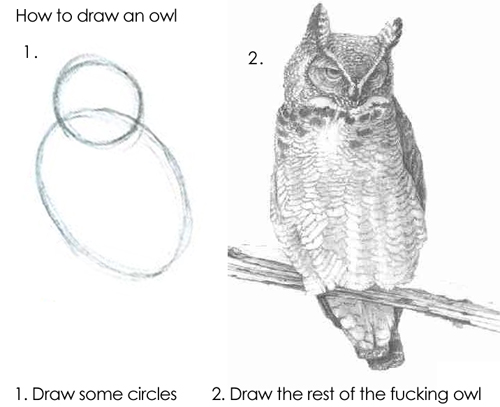
\includegraphics[width=.6\textwidth]{figures/how-to-draw-an-owl}
	\end{figure}
\end{frame}
\subsection{Math notation}
\begin{frame}[label={sec:org00d2d44}]{Notation}

	Let $[K]$ denote the set $\{1, \ldots, K \}$ for a positive integer $K$. Assume
	the data is comprised of iid replicates:

	\begin{equation}
		\left\{{\covarrv}_{\obsindex},\, {\armrv}_{\obsindex},\,
		{\resprv}_{\obsindex} \right\}_{\obsindex = 1}^{\maxobsindex}
	\end{equation}

	where
	\vfill \pause

	\begin{itemize}
		\item $\covarrv_{\obsindex} \in \covarspace \subseteq
			      \symbb{R}^{\dimarmparam}$ denotes the covariates (contexts)

		\item $\armrv_{ \obsindex} \in \armspace$ denotes the treatment arm (arm,
		      intervention, action)

		\item $\resprv_{ \obsindex} \in \symbb{R}$ denotes the response (reward)
	\end{itemize}

	\vfill \pause

	We'll use the potential outcome framework and denote the potential outcome 	$\po(\armobs)$

\end{frame}


\begin{frame}{Operator notation}
	\begin{itemize}
		\item $\covarrv_1, \ldots, \covarrv_{\maxobsindex}$ is an iid random sample from a
		      fixed but unknown distribution $\Pop$
		\item $\genericfun$ is a generic parametric function indexed by $\theta \in \Theta$
		\item $\hat{\theta} \in \Theta$ is a random variable constructed from the sample
		      $\covarrv_1, \ldots, \covarrv_{\maxasymindex}$
	\end{itemize}
	\vfill \pause

	$\Pop$ denotes the probability measure:
	\begin{equation*}
		\Pop \genericfun(\covarrv; \hat{\theta}) = \int \genericfun(\covarobs;\,\widehat{\theta}) \dv
		\Pop(\covarobs))
	\end{equation*}

	\vfill \pause $\Pn$ denotes the corresponding empirical measure:

	\begin{equation*}
		\Pn \genericfun(\covarrv; \hat{\theta}) = \asymindex^{-1}\sum_{i =
			1}^{\asymindex} \genericfun(\covarobs_{i};\,\hat{\theta})
	\end{equation*}
	\vfill \pause

	$\leadsto$ denotes convergence in distribution.

	\vfill
\end{frame}

\subsection{Treatment Policy Notation}

\begin{frame}{Treatment Policy Notation}
	A policy (aka DTR, treatment rule) $\pol$ maps contexts to actions $\pol: \covarspace \mapsto \armspace$.

	\vfill \pause
	The expected response given
	the covariates and arm assignment $\E[\resprv \vert \covarobs, \armobs =
			\armindex]$is given by $\meanfun(\covarobs, \armobs = \armindex) \equiv \meanfunk(x)$
	for some function $\meanfun \in \funclass$.

	\vfill \pause
	Define the value of a policy $\pol$ as
	\begin{equation}
		\val(\pol) = \E_{\covarrv}[\po(\armobs = \pol(\covarrv))]
	\end{equation}

	\vfill \pause
	An optimal policy $\optpol$ is any policy that satisfies
	\begin{equation}
		\val(\optpol) \geq \val(\pol) \qquad \text{for all }\pol \in \polset
	\end{equation}
\end{frame}

\begin{frame}{Value Functions}
	\begin{enumerate}
		\item Conditional Value of the estimated optimal policy

		      $$\val(\polhatn) = \E_{\covarrv}[\polhatn(\covarrv) \vert \polhatn] = \Pop \polhatn(\covarrv)$$

		      \vfill \pause

		\item (Expected) Value of an estimated optimal policy
		      $$\E_{\covarrv}[\polhatn(\covarrv)]$$

		      \vfill \pause

		\item Value of the optimal policy
		      $$\val(\optpol) = \E_{\covarrv}[\optpol(\covarrv)] = \Pop \optpol(\covarrv)$$
	\end{enumerate}

	\vfill \pause

	Will estimators of these functions asymptotically equivalent?

	\vfill \pause
	Brainstorm a scenario for each of the value functions where that estimand
	would 	make the most sense.
\end{frame}


\begin{frame}{The Estimated Optimal Policy}
	Denote the estimated optimal policy $\polhatn$, and to simplify life assume
	that there is a unique maximizer for every covariate value, or more formally

	$$\text{For all} \covarrv \in \covarspace \text{ there exists an arm }k^*
		\text{ such that } \meanfun_{\armindex^*}(\covarrv) > \max_{\armindex \neq
			\armindex^*} \meanfunk(\covarrv)$$

	\vfill \pause
	This assumption ensures that the optimal policy is deterministic:
	$$\polopt(\covarobs) = \argmax_{\armindex \in [\maxarmindex]}\meanfunk(\covarobs)$$

	The estimated optimal policy
\end{frame}


\begin{frame}{Operator Notation Exercise}
	Rewrite the following in operator notation:
	\vfill
	\begin{itemize}

		\item Conditional Value of the estimated optimal policy

		      $$\E_{\covarrv}[\polhatn(\covarrv) \vert \polhatn] = ?$$

		\item Value of the optimal policy
		      $$\E_{\covarrv}[\optpol(\covarrv)] = ?$$

		\item Estimated Value of the optimal policy

		      $$\valhatn(\polhatn(\covarrv)) = ?$$
	\end{itemize}
	\vfill

\end{frame}

\begin{frame}{Operator Notation Exercise}
	Rewrite the following in operator notation:
	\vfill
	\begin{itemize}

		\item Conditional Value of the estimated optimal policy
		      \pause
		      $$\E_{\covarrv}[\polhatn(\covarrv) \vert \polhatn] = \Pop \polhatn(\covarrv)$$
		      \pause
		\item Value of the optimal policy
		      \pause
		      $$\E_{\covarrv}[\optpol(\covarrv)] = \Pop \optpol(\covarrv)$$
		      \pause
		\item Estimated Value of the estimated optimal policy
		      \pause
		      $$\valhatn(\polhatn(\covarrv)) = \Pn \val(\polhatn(\covarrv))$$
	\end{itemize}
	\vfill

\end{frame}


\begin{frame}{Operator Notation Exercise}
	Rewrite the following in operator notation:
	\vfill
	\begin{itemize}

		\item Conditional Value of the estimated optimal policy

		      $$\E_{\covarrv}[\polhatn(\covarrv) \vert \polhatn] = \Pop \polhatn(\covarrv)$$

		\item Value of the optimal policy
		      $$\E_{\covarrv}[\optpol(\covarrv)] = \Pop \optpol(\covarrv)$$
	\end{itemize}
	\vfill

\end{frame}


\section{Nonregular Introduction}
\begin{frame}{Toy Problem: Max of Gaussian Means}
	Suppose we have a random iid sample of size $n$ where
	\begin{equation*}
		X_i \sim \MVN \left(\symbf{\mu} = \begin{pmatrix}2 \\ -1 \end{pmatrix},\, \Sigma = \begin{bmatrix}1 & 0
               \\ 0 & 1\end{bmatrix} \right)
	\end{equation*}

	\vfill
	\pause

	In the general case let $p$ denote the dimension of $\symbf{\mu}$ and assume
	that the covariance matrix is the identity matrix. Suppose we are interested
	in $\theta$:

	$$\theta = \max_{j \in
			[p]} \mu_j = \maxsym_{j = 1}^{p} \mu_j$$
	\vfill

	Here $\theta = \max \{2, -1\} = 2$

	\vfill
	\pause
	Let $$\hat{\theta}_n = \max_{j \in \{1, 2 \}} \Pn {X}_j $$
	\vfill
	\pause
	What is the limiting distribution of $\rootn (\hat{\theta} - \theta)$ for $\symbf{\mu} =
		(2, -1 )^{\trans}$?

	Hint: don't overthink it
\end{frame}

\begin{frame}{Max of Gaussian Means continued}
	A: $\rootn (\hat{\theta} - \theta) \convd \symtt{N}(0, 1)$
	\pause
	\vfill
	Suppose $\symbf{\mu} = (0 , 0)^{\trans}$

	Now what is the limiting distribution of $ \rootn (\hat{\theta} - \theta)$?

	\vfill \pause

	$$\rootn (\hat{\theta} - \theta) \convd \max(\symtt{N}(0, 1), \symtt{N}(0, 1))$$

	Now the limiting distribution is the maximum of two independent standard
	normal RVs.

	\vfill \pause

	Problem: the limiting distribution depends on the value of the parameter
	$\symbf{\mu}$

	\vfill

	To analyze the value function we'll need to address nonregular asymptotics.
\end{frame}

\begin{frame}{Visualizing the Problem --- Fixed $\delta$}
\end{frame}

\begin{frame}{Visualizing the Problem --- Varying $\delta$}
\end{frame}

\begin{frame}{Abstract problem}
	Nonsmooth functional of a smooth function

	Approach overview:

	$m$ out of $n$ directly approximate the nonsmooth functional - let the
	perturbations in $m_n$ be larger than the perturbations from the non-regularlity
\end{frame}

\subsection{Asymptotic Aside}

\begin{frame}{What makes a good approximation?}
	Asymptotically valid does not guarantee a good approximation


	Uncertainty about the set of maximizers needs to be reflected in our
	approximation even if any positive difference results in asymptotic
	normality for $\widehat{\theta}_n$
\end{frame}

\subsection{Local Alternatives}
\begin{frame}{The Local Alternative}
	Idea: decompose into a static part and a part that changes with $n$

	$$\mu_n = \mu_0 + s h(n)$$

	$\mu_0, s \in \mbbR^{p)}$ are both fixed

	$h(n)$, often but not exclusively $n^{-1/2}$, controls the perturbations
\end{frame}

\begin{frame}{Construction a confidence interval}
\end{frame}

\begin{frame}{CI Proof}
\end{frame}



\section{Constructing Asymptotic Confidence Intervals}
\subsection{Projections}
\begin{frame}{Projection Region Big Picture}
	%	Recall our formulation $\theta_n = \theta_0 + h(n)s$
	\begin{itemize}
		\item The empirical estimator $\widehat{\mu}_n = \Pn X$ is well-behaved (regular, asymptotically normal)
		      \vfill \pause
		\item If we knew $\mu_0$ forming confidence intervals for ${\theta}_0$
		      would be simple --- we'd know $\mu_{01}$ is the maximizer and
		      construct a CI for $\mu_{01}$
	\end{itemize}
	\vfill \pause
	Solution:
	\begin{enumerate}
		\item Determine all plausible values of $\mu_0$ using the $(1- \alpha)$ CI
		\item For each plausible value of $\mu_0$, construct a CI for ${\theta}_0$
		      treating the plausible $\mu_0$ as fixed
		\item Take a union over over all of these CIs
	\end{enumerate}
	\vfill \pause
	Can be very conservative

	%	Particularly in the context of DTRs because
\end{frame}

\begin{frame}{Projection Proof}
\end{frame}

\begin{frame}{Adaptive Projection Regions}

\end{frame}
\subsection{Bound-based}
\begin{frame}{Bound-based}
\end{frame}
\subsection{Bootstrap}
\begin{frame}{The $m$-out-of-$n$ Bootstrap}
\end{frame}

\begin{frame}{The Jackknife+}
\end{frame}

\subsection{Conformal Inference}
\begin{frame}{Jackknife+}
\end{frame}
\begin{frame}{What exactly is conformal inference guaranteeing}
\end{frame}
\section{Avoiding Nonregularity}
\begin{frame}{Alternatives to Asymptotics}
	If the blow-up happens in the limit, what if we just don't take it to the limit?
\end{frame}

\begin{frame}{Finite-sample bounds}
	Similar in spirit to the asymptotic bound-based approach, but with Martingales
	playing the role of the nicely behaved functions.

	More specifically test super-martingales. Recall that a super martingale is
	a stochastic process satisfying

	$$\E[Z(\obsindex + s) | Z(\obsindex)] \leq Z(s) \forall \obsindex, s \in \mbbN^+$$

	A test super-martingale $M_t$ is a non-negative super-martingale that under
	the null $\E_{P_0}[M_\obsindex] \leq 1$ at any time $\obsindex$
\end{frame}

\begin{frame}{Additional Notation of Note}
	Let $\histobs_{\obsindex}(\armrv_{\obsindex}, \covarrv_{\obsindex}) =
		\prob(\armrv_{\obsindex} = \armobs \mid \covarrv_{\obsindex} = \covarobs, \histspace_{t-1})$
\end{frame}

\begin{frame}{Assumptions in this Setting}
	$\resprv$ is bounded, and for convenience we'll assume $\resprv \in [0,1]$


	Adapted

	Exogenous

	$$\prob(\armrv_{\obsindex} \mid \histspace_{\obsindex - 1}) =
		\prob(\armrv_{\obsindex} \mid \covarrv_{\obsindex})$$
\end{frame}

\begin{frame}{Confidence Sequences}
	\begin{definition}[Confidence Sequence]
	\end{definition}
\end{frame}

\begin{frame}{Key Result}

\end{frame}

\begin{frame}{Practical Improvements}
	\begin{itemize}
		\item Double robustness
		\item Trimming the observed rewards
		\item Empirical weights
	\end{itemize}
\end{frame}

\begin{frame}{From Sequence to Interval}
	Suppose that all we care about is a $(1 - \alpha)$ CI after $\maxobsindex$
	observations.

	\vfill
	A CS is also trivially a CI at a fixed time, but the width of the interval
	will be wider than if we only needed to guarantee coverage at one point in
	time.

	\vfill \pause

	\begin{lemma}[The minimum and maximum bounds of a $1 - \alpha$ confidence
			sequence form a $1 - \alpha$ confidence interval.] Define lower and upper bounds, $L^{\text{CI}}$ and
		$L^{\text{CI}}$, as
		$$L^{\text{CI}} = \max_{\obsindex \leq \maxobsindex}
			L_{\obsindex}^{\text{CS}} \qquad \text{ and } U^{\text{CI}} = \max_{\obsindex \leq
				\maxobsindex} U_{\obsindex}^{\text{CS}}$$

		Then $(L^{\text{CI}},\, U^{\text{CI}})$ is a $(1 - \alpha)$ confidence
		interval for $\val(\pol)$
	\end{lemma}
\end{frame}

\begin{frame}{What we didn't get to}
	Data-derived policies

	Comparing multiple policies

	Off policy evaluation
\end{frame}
\section{Where Next?}

\begin{frame}{Where to Start}
	\vfill

	Start with Chapter 10 of \cite{tsiatis2019Dynamic}
	\vfill

\end{frame}

\begin{frame}{General Theory -- Asymptotic}
	\vfill
	\begin{itemize}
		\item Chapter 3 of \cite{tsiatis2006Semiparametric}
		      \vfill
		\item Chapters 6 and 7 of \cite{vandervaart2000Asymptotic}
		      \vfill
		\item \cite{kosorok2008Introduction}
		      \vfill
		\item Important Paper: \cite{hirano2012Impossibility}
		      \vfill


		\item 	\cite{bibaut2021PostContextualBandit}
		      \vfill
	\end{itemize}
\end{frame}

\begin{frame}{Precision Medicine}
	\vfill
	\begin{itemize}
		\item \cite{laber2014Dynamic}
		      \vfill

		\item 	\cite{luedtke2016Statistical}
		      \vfill

		\item 	\cite{shi2022Statistical}

		\item \cite{hadad2021Confidence}
	\end{itemize}
	\vfill

\end{frame}

\begin{frame}{General Theory -- Non-asymptotic}
	\vfill
	\begin{itemize}
		\item \cite{waudby-smith2022Anytimevalid}
		      \vfill

		      \item\cite{howard2021Timeuniform}
	\end{itemize}
	\vfill


\end{frame}

\appendix
\printbibliography

\end{document}
%%% Local Variables:
%%% mode: LaTeX
%%% TeX-master: t
%%% End:
